\documentclass{beamer}
\usetheme{Boadilla}


\usepackage[utf8]{inputenc}
\usepackage{caption, subcaption}
\usepackage{amssymb, amsmath}
\usepackage{graphicx}
\usepackage{xcolor}
\usepackage[square, numbers]{natbib}
\bibliographystyle{unsrt}

\DeclareMathOperator*{\argmin}{arg\,min}


\title[Data-driven targeted gene panels]{Data-driven design of targeted gene panels for estimating immunotherapy biomarkers}
\author[Bradley and Cannings]{Jacob R. Bradley, Timothy I. Cannings}
\date{January 2021}
% \institute[]{University of Edinburgh}


\titlegraphic{
\includegraphics[height=.7cm]{figures/mims_logo.png}\hspace*{.5cm}~%

\includegraphics[height=.7cm]{figures/uoe_logo.png}\hspace*{.5cm}~
   
\includegraphics[height=1cm]{figures/igmm_logo.png}
}

\begin{document}

\begin{frame}
\titlepage
\end{frame}

\begin{frame}{Abstract}
\begin{enumerate}[I]
    \item Exome-wide biomarkers such as tumour mutation burden (TMB) are useful predictors of response to immunotherapy.
    \item While whole-exome sequencing directly measures TMB, its cost prevents it from being standard-of-care.
    \item We develop a data-driven framework both for selecting targeted gene panels and for using them to intelligently estimate immunotherapy biomarkers.
    \item To do this, we utilise an exome-wide generative model of mutation, whose structure can be chosen to reflect biological assumptions.
\end{enumerate}
\end{frame}


\begin{frame}
\frametitle{Outline}
\tableofcontents
\end{frame}

\section{Biological/Clinical Background}


\subsection{Cancer and immunotherapy}
\begin{frame}{Cancer is a disease of the genome}
Cancer arises when DNA in cells changes (mutates) \citep{hanahan_hallmarks_2011}.
\begin{figure}[t!]
    \centering
    \begin{subfigure}[t]{0.45\textwidth}
        \centering
        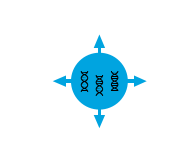
\includegraphics[height=1.5in]{figures/IC1.png}
        \caption{Non-cancer cell: Normal DNA.}
    \end{subfigure}
    ~ 
    \begin{subfigure}[t]{0.45\textwidth}
        \centering
        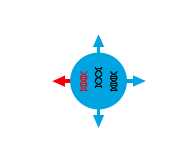
\includegraphics[height=1.5in]{figures/IC2.png}
        \caption{Cancer cell: Mutated DNA.}
    \end{subfigure}
\end{figure}
\end{frame}
\begin{frame}{Immunotherapy enables the immune system}
Immunotherapy 'releases the brakes' on the immune system in order for it to attack tumours \citep{pardoll_blockade_2012}.
\begin{figure}[t!]
    \centering
    \begin{subfigure}[t]{0.45\textwidth}
        \centering
        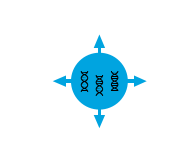
\includegraphics[height=1.5in]{figures/IC1.png}
        \caption{Low-damage cell: \textbf{unrecognisable} to immune system.}
    \end{subfigure}
    ~ 
    \begin{subfigure}[t]{0.45\textwidth}
        \centering
        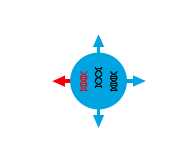
\includegraphics[height=1.5in]{figures/IC2.png}
        \caption{High-damage cell: \textbf{recognisable} to the immune system.}
    \end{subfigure}
\end{figure}
However, the immune system can only attack tumours that it recognises!
\end{frame}

\subsection{Exome-wide biomarkers}


\begin{frame}{Tumour mutation burden stratifies patients for immunotherapy response}
As a simple proxy for likelihood of immune response, we can use \textbf{tumour mutation burden}: the total count of non-synonymous mutations throughout the tumour exome \citep{zhu_association_2019, cao_high_2019}. \\
~\\
Advantages:
\begin{enumerate}[I]
    \item Calculated from DNA sequencing only (compatible with liquid biopsy \citep{gandara_blood-based_2018}).
    \item Relevant across cancer types.
\end{enumerate}
Disadvantages:
\begin{enumerate}[I]
    \item Requires Whole-Exome Sequencing (WES) to measure directly. 
    \item Fails to incorporate other features of the immune environment.
\end{enumerate}



\end{frame}

\subsection{Targeted gene panels}

\begin{frame}{Targeted panels make genomic biomarkers viable}
Rather than the entire exome/genome, targeted gene panels sequence a \textbf{subset} of genes.

\begin{figure}[t!]
    \centering
    \begin{subfigure}[t]{0.45\textwidth}
        \centering
        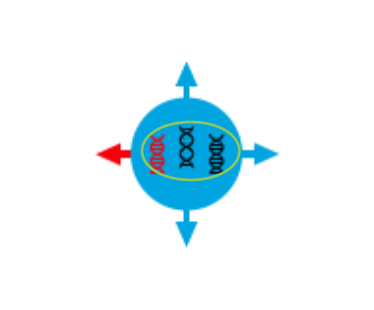
\includegraphics[height=1.5in]{figures/IC5.png}
        \caption{Whole-exome sequencing: \textbf{all genes} sequenced.}
    \end{subfigure}
    ~ 
    \begin{subfigure}[t]{0.45\textwidth}
        \centering
        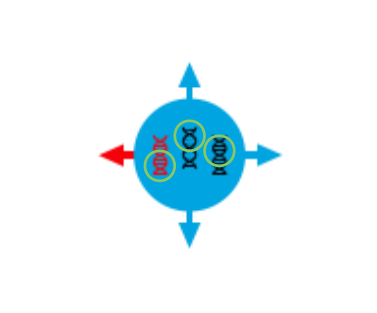
\includegraphics[height=1.5in]{figures/IC6.png}
        \caption{Targeted panel sequencing: \textbf{subset} of genes sequenced.}
    \end{subfigure}
\end{figure}

\end{frame}
\begin{frame}{Problem Statement}
Aims: 

\begin{enumerate}[1]
\item Select a discrete set of genes to form a panel (of pre-specified cost). 
\item Estimate TMB from panel sequencing data.
\end{enumerate} 
~\\
\end{frame}

\begin{frame}{Mutations and biomarkers: some notation}
We'll use $i,g,$ and $s$ to refer to:
\begin{enumerate}
    \item A sample $i$ (ranging from $i=1$ to $i=N$),
    \item A gene $g$ (belonging to some index set $G$),
    \item A variant type $s$ (for example synonymous/non-synonymous).
\end{enumerate}
Finally, we write:
\begin{enumerate}[4]  
    \item $M_{igs}$, to refer to a mutation count of a particular sample, gene, and mutation type.
\end{enumerate} 
~\\
We then can define the TMB of the $i$th sample via:
\[
T_i = \sum_{\substack{g \in G \\ s: \ \text{non-}\\ \text{synonymous}}} M_{igs}.
\]

\end{frame}

\section{Generative/predictive modelling framework}
\subsection{Generative models: what and why?}
\begin{frame}{What is a generative model of mutation?}
A generative model of mutation attempts to capture the \textbf{underlying distribution} of variants across the entire exome/genome. \\
~\\
A simple example (Poisson):
\begin{equation}
    M_{igs} \sim \mathrm{Poisson}(\lambda_{gs})
\end{equation}
\end{frame}

\begin{frame}{Why use generative models of mutation?}

\begin{enumerate}[I]
    \item Utilise known biology to inform the structure of the model.
\end{enumerate}
~\\
\begin{enumerate}[II]
    \item (Sometimes) make interpretable inferences.
\end{enumerate}
~\\
\begin{enumerate}[III]    
    \item Generate trust that we've thought about it!  
\end{enumerate}
\end{frame}

\begin{frame}{Why use generative models of mutation?}

\begin{enumerate}[I]
    \item Utilise known biology to inform the structure of the model.
\end{enumerate}
\indent \color{red} Choice of distribution, exome organisation, parameter space.\color{black}
\begin{enumerate}[II]
    \item (Sometimes) make interpretable inferences.
\end{enumerate}
~\\
\begin{enumerate}[III]    
    \item Generate trust that we've thought about it!  
\end{enumerate}
\end{frame}

\begin{frame}{Why use generative models of mutation?}
\begin{enumerate}[I]
    \item Utilise known biology to inform the structure of the model.
\end{enumerate}
~\\
\begin{enumerate}[II]
    \item (Sometimes) make interpretable inferences.
\end{enumerate}
\indent \color{red} Parameter estimates, post-model inference.\color{black}
\begin{enumerate}[III]    
    \item Generate trust that we've thought about it!  
\end{enumerate}
\end{frame}


\subsection{From generative models to predictive models}
\begin{frame}{Generative models to predictive models}
Aims: 

\begin{enumerate}[1]
\item Select a discrete set of genes to form a panel (of pre-specified cost). 
\item A mechanism for estimating TMB from panel sequencing data.
\end{enumerate} 
~\\
Proposed mechanism: Linear estimator.

\begin{equation}
    \hat{T} = \sum_{g,s} w_{gs} M_{igs}
\end{equation}

Optimisation procedure:
\begin{equation}
    \hat{w} := \argmin_w \{ \mathbb{E}[(\hat{T}_i - T_i)^2] + \lambda |w|\},
\end{equation}
where $\lambda$ is a penalty specifying panel cost, and the expectation $\mathbb{E}$ is over the distribution learned by our generative model.
\end{frame}



\section{Application to non-small cell lung cancer}

\begin{frame}{NSCLC: Generative Model Structure}

\end{frame}

\begin{frame}{NSCLC: Poisson-based generative model fit}

\begin{figure}[htbp]
\centering
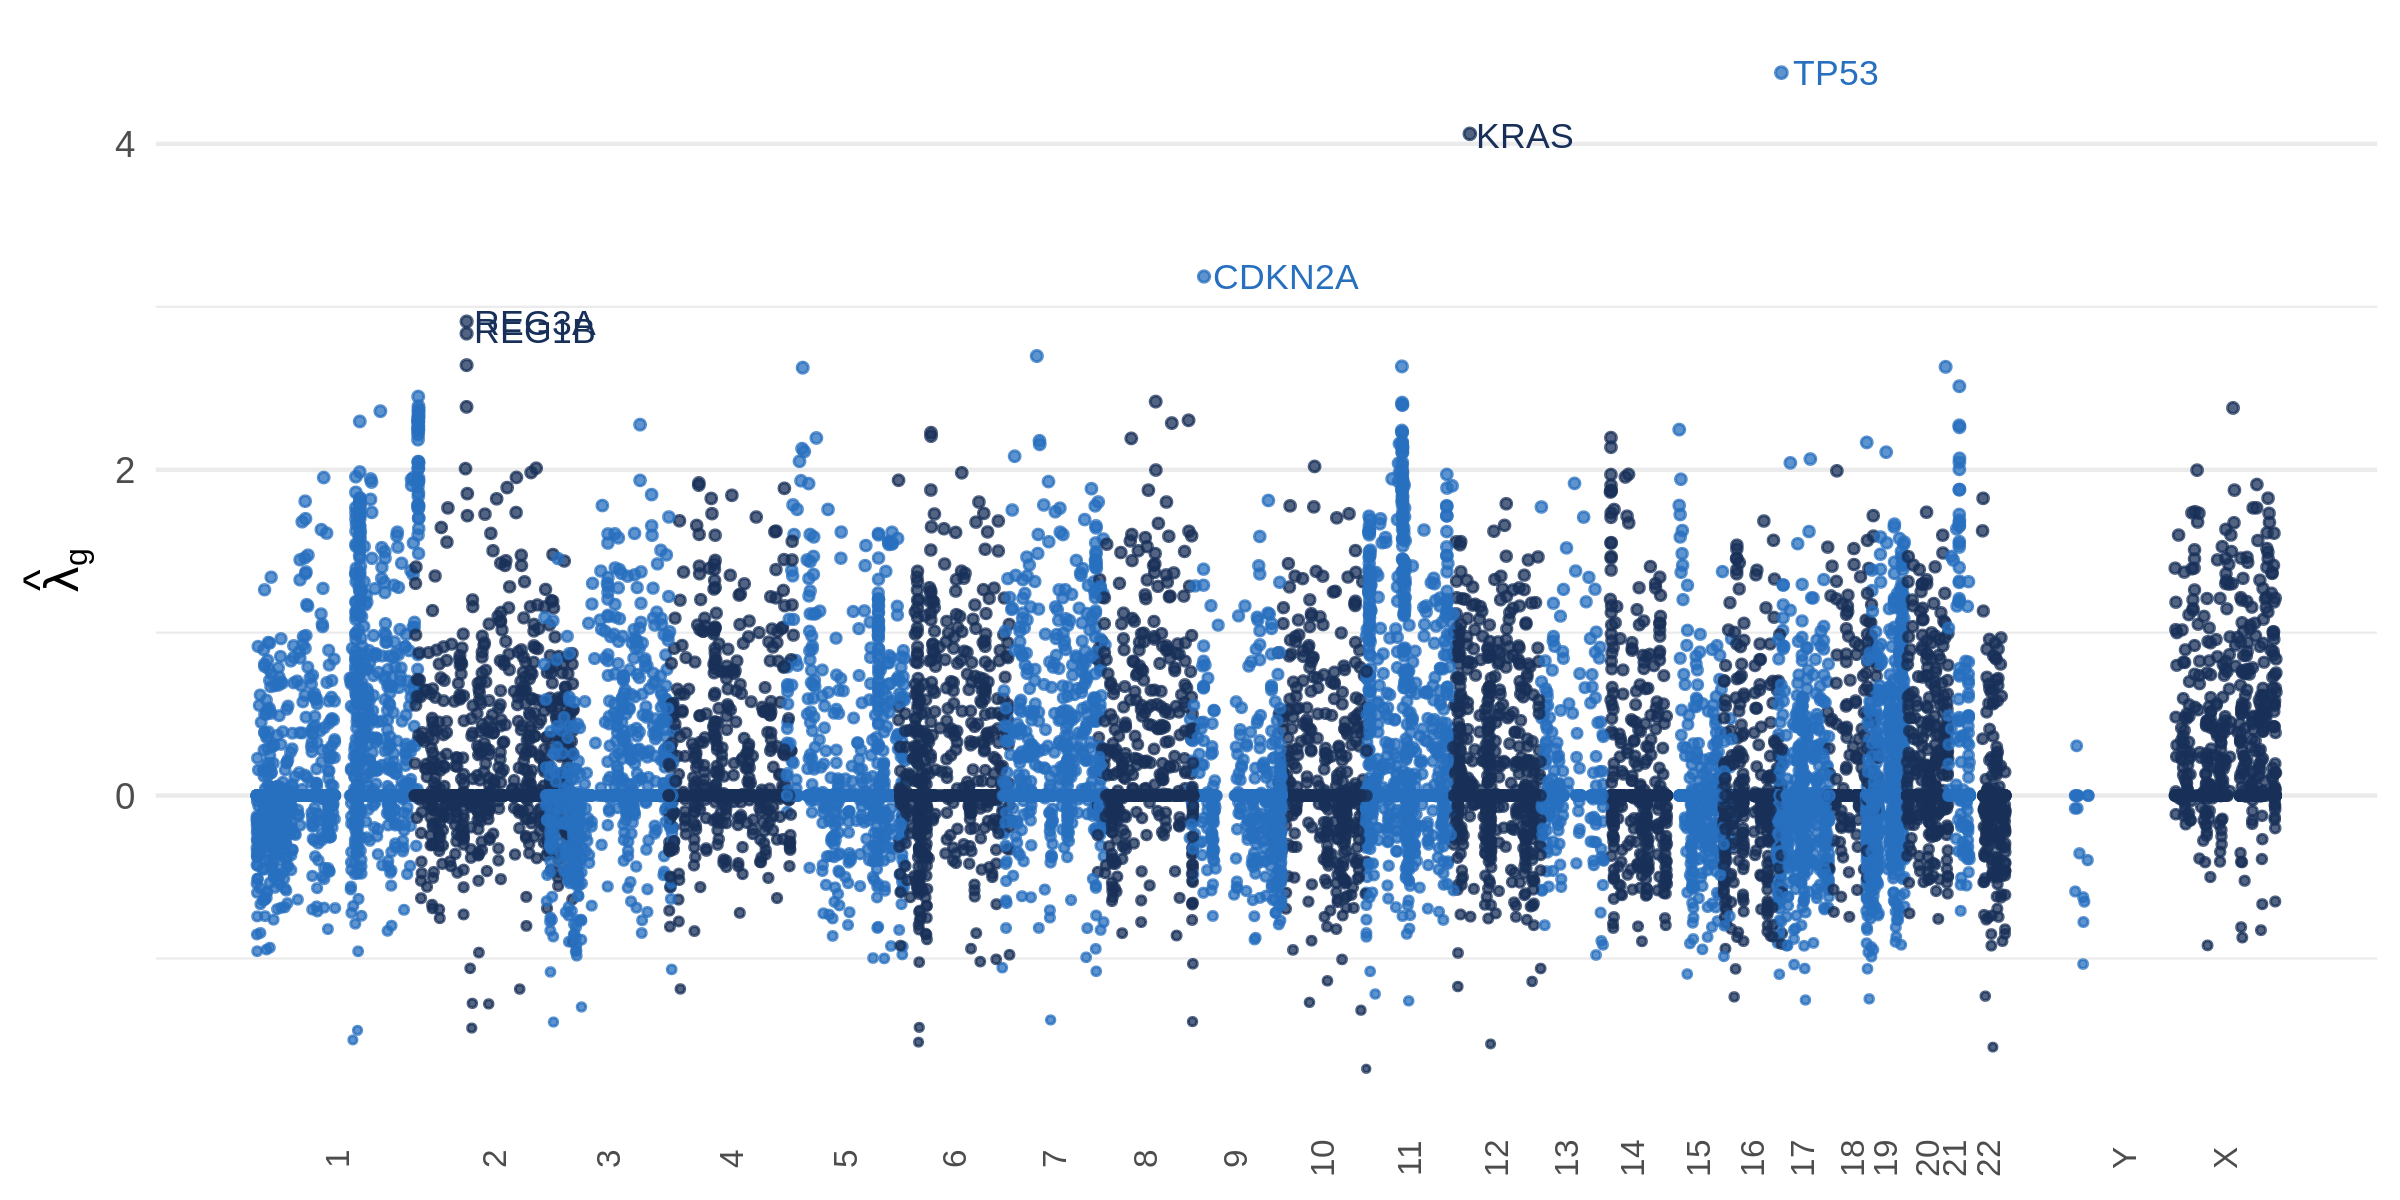
\includegraphics[width=4in]{figures/fig4.png}
\caption{Generative model parameters. \citep{bradley_data-driven_2021}\label{fig:3}}
\end{figure}
\end{frame}

\begin{frame}{NSCLC: Poisson-based generative model fit}

\begin{figure}[htbp]
\centering
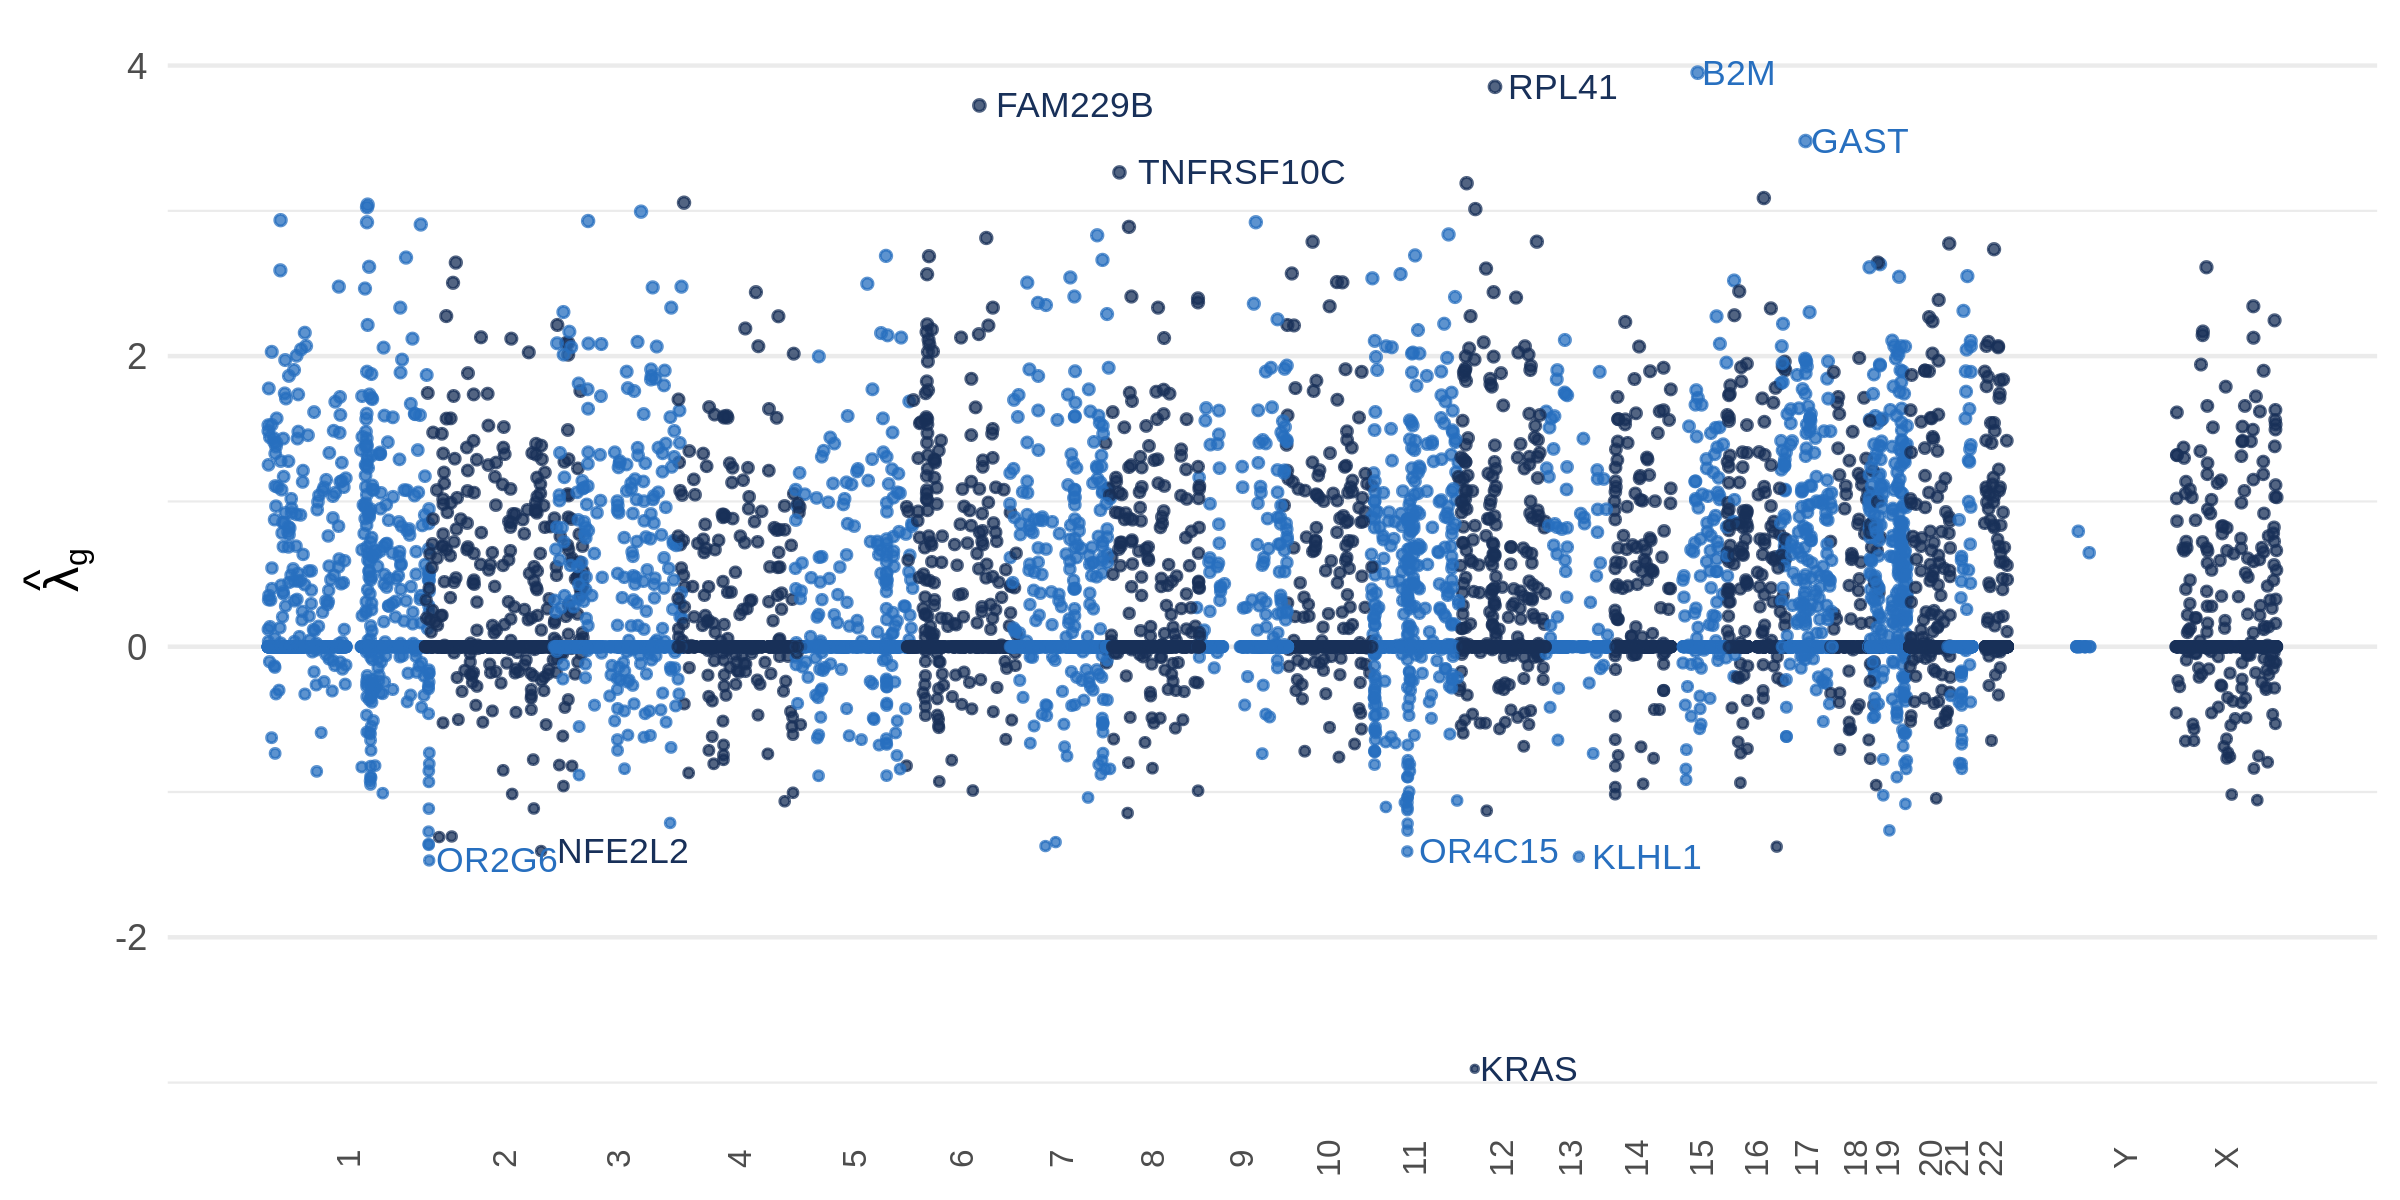
\includegraphics[width=4in]{figures/fig5.png}
\caption{Generative model parameters (indel-specific) \citep{bradley_data-driven_2021}. \label{fig:3}}
\end{figure}
    
\end{frame}

\begin{frame}{NSCLC: Estimation performance}

\begin{figure}[htbp]
\centering
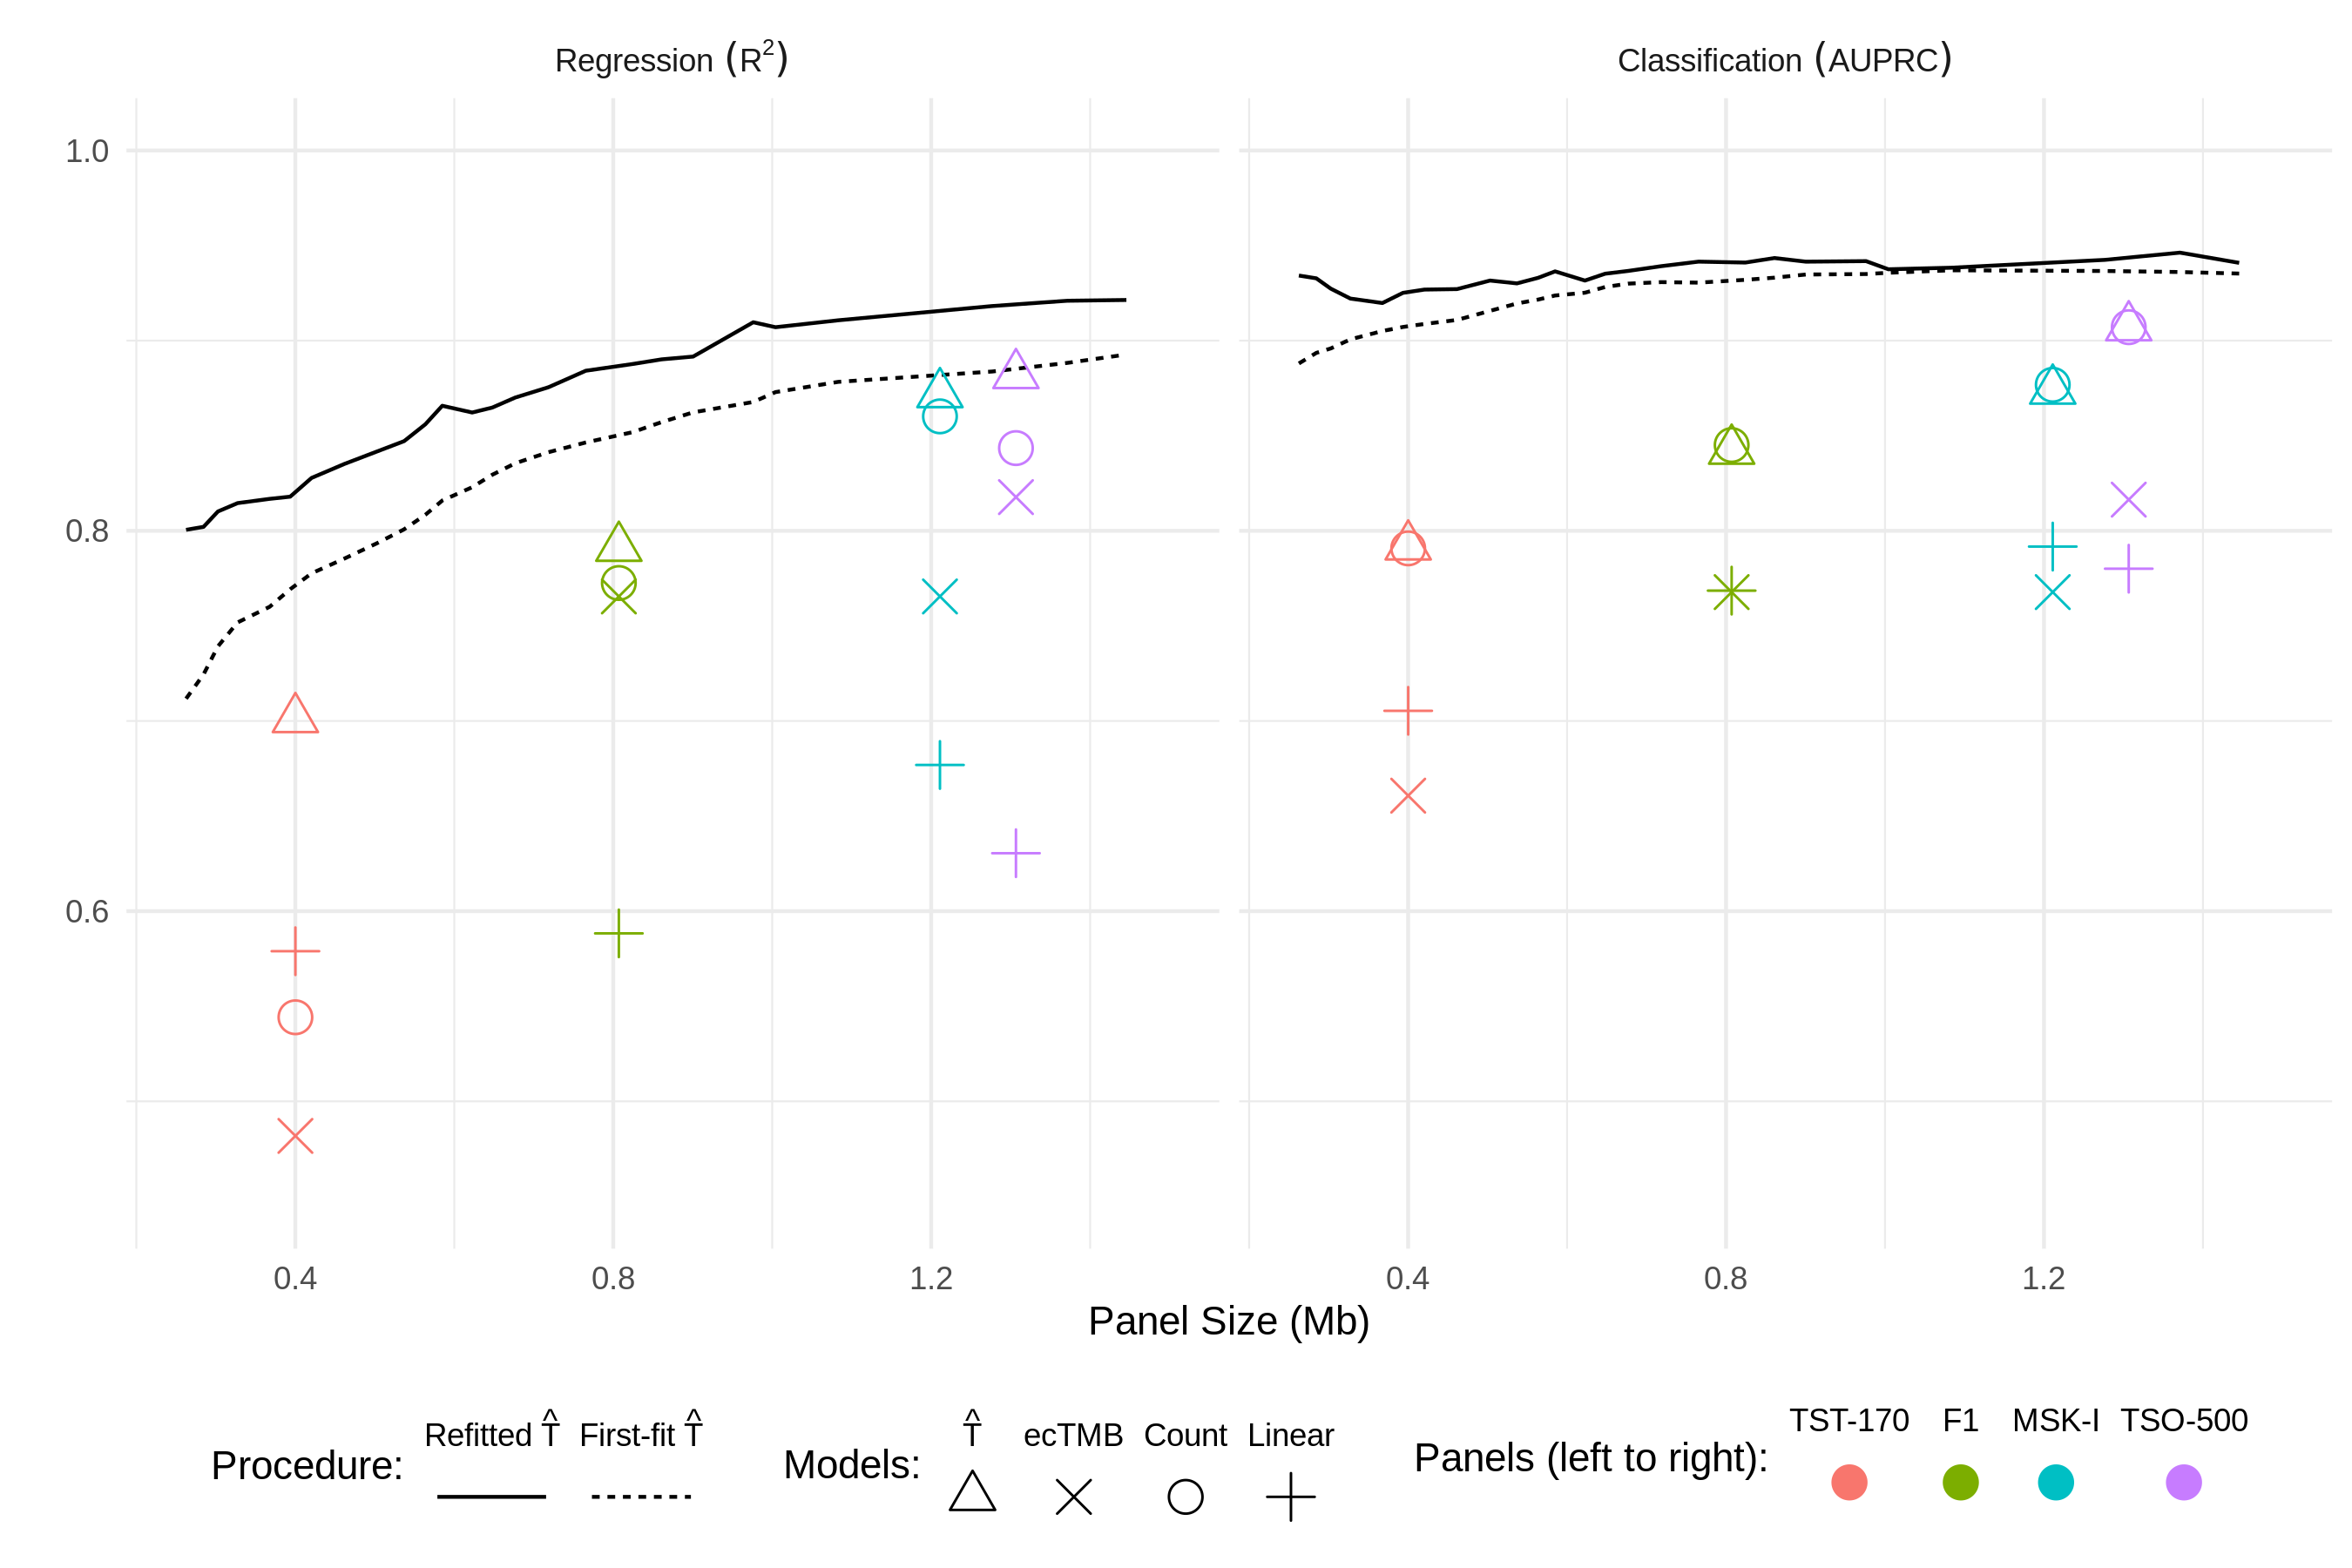
\includegraphics[width=4in]{fig7.png}
\caption{Predictive model performance: comparison with commercial panels and other predictive methods \citep{bradley_data-driven_2021, yao_ectmb_2020}. \label{fig:7}}
\end{figure}
\end{frame}

\begin{frame}[allowframebreaks]
        \frametitle{References}
        \bibliography{zotero-refs.bib}
\end{frame}

\end{document}